%% bare_conf_compsoc.tex
%% V1.4b
%% 2015/08/26
%% by Michael Shell
%% See:
%% http://www.michaelshell.org/
%% for current contact information.
%%
%% This is a skeleton file demonstrating the use of IEEEtran.cls
%% (requires IEEEtran.cls version 1.8b or later) with an IEEE Computer
%% Society conference paper.
%%
%% Support sites:
%% http://www.michaelshell.org/tex/ieeetran/
%% http://www.ctan.org/pkg/ieeetran
%% and
%% http://www.ieee.org/

%%*************************************************************************
%% Legal Notice:
%% This code is offered as-is without any warranty either expressed or
%% implied; without even the implied warranty of MERCHANTABILITY or
%% FITNESS FOR A PARTICULAR PURPOSE! 
%% User assumes all risk.
%% In no event shall the IEEE or any contributor to this code be liable for
%% any damages or losses, including, but not limited to, incidental,
%% consequential, or any other damages, resulting from the use or misuse
%% of any information contained here.
%%
%% All comments are the opinions of their respective authors and are not
%% necessarily endorsed by the IEEE.
%%
%% This work is distributed under the LaTeX Project Public License (LPPL)
%% ( http://www.latex-project.org/ ) version 1.3, and may be freely used,
%% distributed and modified. A copy of the LPPL, version 1.3, is included
%% in the base LaTeX documentation of all distributions of LaTeX released
%% 2003/12/01 or later.
%% Retain all contribution notices and credits.
%% ** Modified files should be clearly indicated as such, including  **
%% ** renaming them and changing author support contact information. **
%%*************************************************************************


% *** Authors should verify (and, if needed, correct) their LaTeX system  ***
% *** with the testflow diagnostic prior to trusting their LaTeX platform ***
% *** with production work. The IEEE's font choices and paper sizes can   ***
% *** trigger bugs that do not appear when using other class files.       ***                          ***
% The testflow support page is at:
% http://www.michaelshell.org/tex/testflow/



\documentclass[conference]{IEEEtran}
% Some/most Computer Society conferences require the compsoc mode option,
% but others may want the standard conference format.
%
% If IEEEtran.cls has not been installed into the LaTeX system files,
% manually specify the path to it like:
% \documentclass[conference,compsoc]{../sty/IEEEtran}





% Some very useful LaTeX packages include:
% (uncomment the ones you want to load)


% *** MISC UTILITY PACKAGES ***
%
%\usepackage{ifpdf}
% Heiko Oberdiek's ifpdf.sty is very useful if you need conditional
% compilation based on whether the output is pdf or dvi.
% usage:
% \ifpdf
%   % pdf code
% \else
%   % dvi code
% \fi
% The latest version of ifpdf.sty can be obtained from:
% http://www.ctan.org/pkg/ifpdf
% Also, note that IEEEtran.cls V1.7 and later provides a builtin
% \ifCLASSINFOpdf conditional that works the same way.
% When switching from latex to pdflatex and vice-versa, the compiler may
% have to be run twice to clear warning/error messages.






% *** CITATION PACKAGES ***
%
\ifCLASSOPTIONcompsoc
  % IEEE Computer Society needs nocompress option
  % requires cite.sty v4.0 or later (November 2003)
  \usepackage[nocompress]{cite}
\else
  % normal IEEE
  \usepackage{cite}
\fi
% cite.sty was written by Donald Arseneau
% V1.6 and later of IEEEtran pre-defines the format of the cite.sty package
% \cite{} output to follow that of the IEEE. Loading the cite package will
% result in citation numbers being automatically sorted and properly
% "compressed/ranged". e.g., [1], [9], [2], [7], [5], [6] without using
% cite.sty will become [1], [2], [5]--[7], [9] using cite.sty. cite.sty's
% \cite will automatically add leading space, if needed. Use cite.sty's
% noadjust option (cite.sty V3.8 and later) if you want to turn this off
% such as if a citation ever needs to be enclosed in parenthesis.
% cite.sty is already installed on most LaTeX systems. Be sure and use
% version 5.0 (2009-03-20) and later if using hyperref.sty.
% The latest version can be obtained at:
% http://www.ctan.org/pkg/cite
% The documentation is contained in the cite.sty file itself.
%
% Note that some packages require special options to format as the Computer
% Society requires. In particular, Computer Society  papers do not use
% compressed citation ranges as is done in typical IEEE papers
% (e.g., [1]-[4]). Instead, they list every citation separately in order
% (e.g., [1], [2], [3], [4]). To get the latter we need to load the cite
% package with the nocompress option which is supported by cite.sty v4.0
% and later.





% *** GRAPHICS RELATED PACKAGES ***
%
\ifCLASSINFOpdf
  % \usepackage[pdftex]{graphicx}
  % declare the path(s) where your graphic files are
  % \graphicspath{{../pdf/}{../jpeg/}}
  % and their extensions so you won't have to specify these with
  % every instance of \includegraphics
  % \DeclareGraphicsExtensions{.pdf,.jpeg,.png}
\else
  % or other class option (dvipsone, dvipdf, if not using dvips). graphicx
  % will default to the driver specified in the system graphics.cfg if no
  % driver is specified.
  % \usepackage[dvips]{graphicx}
  % declare the path(s) where your graphic files are
  % \graphicspath{{../eps/}}
  % and their extensions so you won't have to specify these with
  % every instance of \includegraphics
  % \DeclareGraphicsExtensions{.eps}
\fi
% graphicx was written by David Carlisle and Sebastian Rahtz. It is
% required if you want graphics, photos, etc. graphicx.sty is already
% installed on most LaTeX systems. The latest version and documentation
% can be obtained at: 
% http://www.ctan.org/pkg/graphicx
% Another good source of documentation is "Using Imported Graphics in
% LaTeX2e" by Keith Reckdahl which can be found at:
% http://www.ctan.org/pkg/epslatex
%
% latex, and pdflatex in dvi mode, support graphics in encapsulated
% postscript (.eps) format. pdflatex in pdf mode supports graphics
% in .pdf, .jpeg, .png and .mps (metapost) formats. Users should ensure
% that all non-photo figures use a vector format (.eps, .pdf, .mps) and
% not a bitmapped formats (.jpeg, .png). The IEEE frowns on bitmapped formats
% which can result in "jaggedy"/blurry rendering of lines and letters as
% well as large increases in file sizes.
%
% You can find documentation about the pdfTeX application at:
% http://www.tug.org/applications/pdftex





% *** MATH PACKAGES ***
%
%\usepackage{amsmath}
% A popular package from the American Mathematical Society that provides
% many useful and powerful commands for dealing with mathematics.
%
% Note that the amsmath package sets \interdisplaylinepenalty to 10000
% thus preventing page breaks from occurring within multiline equations. Use:
%\interdisplaylinepenalty=2500
% after loading amsmath to restore such page breaks as IEEEtran.cls normally
% does. amsmath.sty is already installed on most LaTeX systems. The latest
% version and documentation can be obtained at:
% http://www.ctan.org/pkg/amsmath





% *** SPECIALIZED LIST PACKAGES ***
%
%\usepackage{algorithmic}
% algorithmic.sty was written by Peter Williams and Rogerio Brito.
% This package provides an algorithmic environment fo describing algorithms.
% You can use the algorithmic environment in-text or within a figure
% environment to provide for a floating algorithm. Do NOT use the algorithm
% floating environment provided by algorithm.sty (by the same authors) or
% algorithm2e.sty (by Christophe Fiorio) as the IEEE does not use dedicated
% algorithm float types and packages that provide these will not provide
% correct IEEE style captions. The latest version and documentation of
% algorithmic.sty can be obtained at:
% http://www.ctan.org/pkg/algorithms
% Also of interest may be the (relatively newer and more customizable)
% algorithmicx.sty package by Szasz Janos:
% http://www.ctan.org/pkg/algorithmicx




% *** ALIGNMENT PACKAGES ***
%
%\usepackage{array}
% Frank Mittelbach's and David Carlisle's array.sty patches and improves
% the standard LaTeX2e array and tabular environments to provide better
% appearance and additional user controls. As the default LaTeX2e table
% generation code is lacking to the point of almost being broken with
% respect to the quality of the end results, all users are strongly
% advised to use an enhanced (at the very least that provided by array.sty)
% set of table tools. array.sty is already installed on most systems. The
% latest version and documentation can be obtained at:
% http://www.ctan.org/pkg/array


% IEEEtran contains the IEEEeqnarray family of commands that can be used to
% generate multiline equations as well as matrices, tables, etc., of high
% quality.




% *** SUBFIGURE PACKAGES ***
% \ifCLASSOPTIONcompsoc
%  \usepackage[caption=false,font=footnotesize,labelfont=sf,textfont=sf]{subfig}
% \else
%  \usepackage[caption=false,font=footnotesize]{subfig}
% \fi
% subfig.sty, written by Steven Douglas Cochran, is the modern replacement
% for subfigure.sty, the latter of which is no longer maintained and is
% incompatible with some LaTeX packages including fixltx2e. However,
% subfig.sty requires and automatically loads Axel Sommerfeldt's caption.sty
% which will override IEEEtran.cls' handling of captions and this will result
% in non-IEEE style figure/table captions. To prevent this problem, be sure
% and invoke subfig.sty's "caption=false" package option (available since
% subfig.sty version 1.3, 2005/06/28) as this is will preserve IEEEtran.cls
% handling of captions.
% Note that the Computer Society format requires a sans serif font rather
% than the serif font used in traditional IEEE formatting and thus the need
% to invoke different subfig.sty package options depending on whether
% compsoc mode has been enabled.
%
% The latest version and documentation of subfig.sty can be obtained at:
% http://www.ctan.org/pkg/subfig




% *** FLOAT PACKAGES ***
%
%\usepackage{fixltx2e}
% fixltx2e, the successor to the earlier fix2col.sty, was written by
% Frank Mittelbach and David Carlisle. This package corrects a few problems
% in the LaTeX2e kernel, the most notable of which is that in current
% LaTeX2e releases, the ordering of single and double column floats is not
% guaranteed to be preserved. Thus, an unpatched LaTeX2e can allow a
% single column figure to be placed prior to an earlier double column
% figure.
% Be aware that LaTeX2e kernels dated 2015 and later have fixltx2e.sty's
% corrections already built into the system in which case a warning will
% be issued if an attempt is made to load fixltx2e.sty as it is no longer
% needed.
% The latest version and documentation can be found at:
% http://www.ctan.org/pkg/fixltx2e


\usepackage{stfloats}
% stfloats.sty was written by Sigitas Tolusis. This package gives LaTeX2e
% the ability to do double column floats at the bottom of the page as well
% as the top. (e.g., "\begin{figure*}[!b]" is not normally possible in
% LaTeX2e). It also provides a command:
%\fnbelowfloat
% to enable the placement of footnotes below bottom floats (the standard
% LaTeX2e kernel puts them above bottom floats). This is an invasive package
% which rewrites many portions of the LaTeX2e float routines. It may not work
% with other packages that modify the LaTeX2e float routines. The latest
% version and documentation can be obtained at:
% http://www.ctan.org/pkg/stfloats
% Do not use the stfloats baselinefloat ability as the IEEE does not allow
% \baselineskip to stretch. Authors submitting work to the IEEE should note
% that the IEEE rarely uses double column equations and that authors should try
% to avoid such use. Do not be tempted to use the cuted.sty or midfloat.sty
% packages (also by Sigitas Tolusis) as the IEEE does not format its papers in
% such ways.
% Do not attempt to use stfloats with fixltx2e as they are incompatible.
% Instead, use Morten Hogholm'a dblfloatfix which combines the features
% of both fixltx2e and stfloats:
%
% \usepackage{dblfloatfix}
% The latest version can be found at:
% http://www.ctan.org/pkg/dblfloatfix



% *** PDF, URL AND HYPERLINK PACKAGES ***
%
%\usepackage{url}
% url.sty was written by Donald Arseneau. It provides better support for
% handling and breaking URLs. url.sty is already installed on most LaTeX
% systems. The latest version and documentation can be obtained at:
% http://www.ctan.org/pkg/url
% Basically, \url{my_url_here}.




% *** Do not adjust lengths that control margins, column widths, etc. ***
% *** Do not use packages that alter fonts (such as pslatex).         ***
% There should be no need to do such things with IEEEtran.cls V1.6 and later.
% (Unless specifically asked to do so by the journal or conference you plan
% to submit to, of course. )
\usepackage{tikz}
\usetikzlibrary{fit,backgrounds,positioning,calc,patterns,snakes} % <- added

%% for proof trees
\newcommand{\rulehskip}{\hskip 1.5em}
\newcommand{\rulevspace}{\vspace{1em}}

% set notation
\newcommand{\set}[1]{\{ #1 \}}

% tuple with angle brackets
\newcommand{\tup}[1]{\langle #1 \rangle}

% semantics brackets
\newcommand{\sem}[1]{\llbracket #1 \rrbracket}

% equality by definition
\newcommand{\defeq}{\triangleq}

% function arrow
\newcommand{\fun}{\rightarrow}

% partial function arrow
\newcommand{\pfun}{\rightharpoonup}

% sequential composition
\newcommand{\seq}{;}

% power set
\newcommand{\pwset}[1]{\mathcal{P}(#1)}

% prefix 
\newcommand{\prefix}[1]{\lceil #1 \rceil}

% function-to-relation
\newcommand{\frel}[1]{#1^\uparrow}

% epsilon/empty 
\newcommand{\eps}{\epsilon}

% some math sets
\newcommand{\N}{{\mathbb{N}}}
\newcommand{\Z}{{\mathbb{Z}}}
\newcommand{\Q}{{\mathbb{Q}}}

% domain/codomain notation
\newcommand{\dom}[1]{\textit{dom}{({#1})}}
\newcommand{\codom}[1]{\textit{codom}{({#1})}}

%\newcommand{\implies}{{\Rightarrow}}
\renewcommand{\iff}{{\Leftrightarrow}}

% check-mark and cross-mark
\newcommand{\cmark}{\text{\color{green!50!black}\ding{51}}}
\newcommand{\xmark}{\text{\color{red!50!black}\ding{55}}}

\newcommand{\instrvdist}{0.75cm}
\newcommand{\instrhdist}{1.1cm}

%% abbrevations

\newcommand{\ie}{\emph{i.e.,} }
\newcommand{\eg}{\emph{e.g.,} }
\newcommand{\etc}{\emph{etc.} }
\newcommand{\sth}{\emph{s.t.} }
\newcommand{\etal}{\emph{et~al.} }
\newcommand{\wrt}{\emph{w.r.t.} }
\newcommand{\aka}{\emph{a.k.a.} }

% event set
\newcommand{\lE}{{\mathtt{E}}}
\newcommand{\lEi}[1]{\lE_{#1}}
\newcommand{\lEo}{\lEi{0}}
\newcommand{\lEs}{\widehat{{\mathtt{E}}}}
\newcommand{\lEsi}[1]{\lEs_{#1}}
\newcommand{\lEso}{\lEsi{0}}
\newcommand{\lR}{{\mathtt{R}}}
\newcommand{\lW}{{\mathtt{W}}}
\newcommand{\lF}{{\mathtt{F}}}
\newcommand{\lTS}{{\mathtt{TS}}}

\newcommand{\lX}{{\mathtt{X}}}

\newcommand{\lEsqeq}[1]{{\lE^{\sqsupseteq#1}}}
\newcommand{\lRsqeq}[1]{{\lR^{\sqsupseteq#1}}}
\newcommand{\lWsqeq}[1]{{\lW^{\sqsupseteq#1}}}
\newcommand{\lFsqeq}[1]{{\lF^{\sqsupseteq#1}}}

% various common domains
\newcommand{\Prog}{\mathsf{Prog}}
\newcommand{\Inst}{\mathsf{Instr}}
\newcommand{\Tid}{\mathsf{Tid}}
\newcommand{\Reg}{\mathsf{Reg}}
\newcommand{\Loc}{\mathsf{Loc}}
\newcommand{\Val}{\mathsf{Val}}
\newcommand{\Bool}{\mathsf{Bool}}
\newcommand{\BinOp}{\mathsf{BinOp}}
\newcommand{\Lab}{\mathsf{Lab}}
\newcommand{\Mod}{\mathsf{Mod}}
\newcommand{\Cont}{\kappa}
\newcommand{\Scp}{\mathsf{Scope}}
\newcommand{\Path}{\pi}
\newcommand{\ThrdState}{\mathsf{ThrdState}}

% labeling of events
\newcommand{\lLAB}{{\mathtt{lab}}}
\newcommand{\lTID}{{\mathtt{tid}}}
\newcommand{\lTYP}{{\mathtt{typ}}}
\newcommand{\lLOC}{{\mathtt{loc}}}
\newcommand{\lMOD}{{\mathtt{mod}}}
\newcommand{\lVALR}{{\mathtt{val_r}}}
\newcommand{\lVALW}{{\mathtt{val_w}}}

\newcommand{\rlab}[2]{\lR({#1},{#2})}
\newcommand{\wlab}[2]{\lW({#1},{#2})}
\newcommand{\flab}{\lF}

\newcommand{\tslab}[1]{\lTS{#1}}

% maps
\newcommand{\regmap}{\sigma}
\newcommand{\thrdmap}{\Sigma}
\newcommand{\appmap}[2]{#1(#2)}
\newcommand{\updmap}[3]{#1[#2 \mapsto #3]}

% instruction pointer
\newcommand{\ip}[1]{#1}

% length
\newcommand{\len}{\mathsf{len}}

% small-step semantics
\newcommand{\thrdst}{s}
\newcommand{\thrdsti}{s_{\mathsf{init}}}
\newcommand{\thrdstep}[1]{\xrightarrow{#1}}
\newcommand{\esstep}[1]{\xhookrightarrow{#1}}
\newcommand{\fullstep}[1]{\xRightarrow{#1}}

% some math notations for event structures
\newcommand{\eventSet}{E}
\newcommand{\eventSeq}{\mathcal{E}}
\newcommand{\caOrd}{\leqslant}
\newcommand{\cfRel}{\#}
\newcommand{\primcfRel}{\sim_{\#}}
\newcommand{\identOrd}{\prec}
\newcommand{\identOrdDual}{\succ}
\newcommand{\identOrdRefl}{\preceq}

\newcommand{\first}{\mathsf{first}}
\newcommand{\fresh}{\mathsf{fresh}}

% some predefined relations
\colorlet{colorPO}{gray!60!black}
\colorlet{colorRF}{green!60!black}
\colorlet{colorCF}{red!60!black}
\colorlet{colorMO}{orange!60!black}
\colorlet{colorRB}{purple}
\colorlet{colorECO}{red!80!black}
\colorlet{colorRSEQ}{cyan}
\colorlet{colorRELP}{cyan}
\colorlet{colorSW}{blue!40!black}
\colorlet{colorHB}{blue}
\colorlet{colorSCB}{violet}
\colorlet{colorPSC}{violet}
\colorlet{colorFSC}{violet}
\colorlet{colorSC}{violet}
\colorlet{colorCA}{gray!60!black}
\colorlet{colorDEPS}{violet!60!black}

\newcommand{\lPO}{{\color{colorPO}\mathtt{po}}}
\newcommand{\lRF}{{\color{colorRF}\mathtt{rf}}}
\newcommand{\lCF}{{\color{colorCF}\mathtt{cf}}}
\newcommand{\lMO}{{\color{colorMO}\mathtt{mo}}}
\newcommand{\lRB}{{\color{colorRB}\mathtt{rb}}}
\newcommand{\lECO}{{\color{colorECO}\mathtt{eco}}}
\newcommand{\lRSEQ}{{\color{colorRSEQ}\mathtt{rseq}}}
\newcommand{\lRELP}{{\color{colorRELP}\mathtt{relp}}}
\newcommand{\lSW}{{\color{colorSW}\mathtt{sw}}}
\newcommand{\lHB}{{\color{colorHB}\mathtt{hb}}}
\newcommand{\lSCB}{{\color{colorSCB} \mathtt{scb}}}
\newcommand{\lPSCB}{\lPSC_{\rm base}}
\newcommand{\lPSCF}{\lPSC_\lF}
\newcommand{\lFSC}{{\color{colorFSC}\mathtt{fsc}}}
\newcommand{\lPSC}{{\color{colorPSC}\mathtt{psc}}}
\newcommand{\lSC}{{\color{colorSC}\mathtt{sc}}}
\newcommand{\lCA}{{\color{colorCA}\mathtt{ca}}}
\newcommand{\lCTRL}{{{\color{colorDEPS}\mathtt{ctrl}}}}
\newcommand{\lDATA}{{{\color{colorDEPS}\mathtt{data}}}}
\newcommand{\lADDR}{{{\color{colorDEPS}\mathtt{addr}}}}
\newcommand{\lCASDEP}{{{\color{colorDEPS}\mathtt{casdep}}}}
\newcommand{\lDEPS}{{\color{colorDEPS}\mathtt{dep}}}

\newcommand{\lmakeE}[1]{#1\mathtt{e}}
\newcommand{\lRFE}{\lmakeE{\lRF}}
\newcommand{\lMOE}{\lmakeE{\lMO}}
\newcommand{\lRBE}{\lmakeE{\lRB}}

\newcommand{\lmakeI}[1]{#1\mathtt{i}}
\newcommand{\lRFI}{\lmakeI{\lRF}}
\newcommand{\lMOI}{\lmakeI{\lMO}}
\newcommand{\lRBI}{\lmakeI{\lRB}}

\newcommand{\lmakeLoc}[1]{#1_{|loc}}

%% functional versions of relations
\newcommand{\lfPO}{f_{\lPO}}
\newcommand{\lfRF}{f_{\lRF}}

%% memory orders
\newcommand{\na}{\mathtt{na}}
\newcommand{\pln}{\mathtt{pln}}
\newcommand{\rlx}{\mathtt{rlx}}
\newcommand{\rel}{{\mathtt{rel}}}
\newcommand{\acq}{{\mathtt{acq}}}
\newcommand{\con}{{\mathtt{con}}}
\newcommand{\acqrel}{{\mathtt{acqrel}}}
\newcommand{\relAcq}{\acqrel}
\newcommand{\sco}{{\mathtt{sc}}}

%% tikz stuff
\newcommand{\event}[3]{#1#2#3}
\tikzset{
   every path/.style={>=stealth},
   po/.style={->,color=colorPO,,shorten >=-0.5mm,shorten <=-0.5mm},
   por/.style={->,color=red,shorten >=-0.5mm,shorten <=-0.5mm},
   ppo/.style={->,color=colorPPO,,shorten >=-0.5mm,shorten <=-0.5mm},
   cf/.style={-,snake=zigzag,segment amplitude=1pt,segment length=3pt,colorCF},
   rmw/.style={->,color=colorRMW,,shorten >=-0.5mm,shorten <=-0.5mm},
   ca/.style={->,color=colorPO,thick,shorten >=-0.5mm,shorten <=-0.5mm},
   rf/.style={->,color=colorRF,dashed,,shorten >=-0.5mm,shorten <=-0.5mm},
   rfs/.style={->,color=colorRF,thick,dashed,,shorten >=-0.5mm,shorten <=-0.5mm},
   rb/.style={->,color=colorRB,thick,shorten >=-0.5mm,shorten <=-0.5mm},
   cc/.style={->,color=colorCC,thick,shorten >=-0.5mm,shorten <=-0.5mm},
   ew/.style={<->,color=colorEW,dotted,thick,shorten >=-0.5mm,shorten <=-0.5mm},
   mo/.style={->,color=colorMO,dotted,thick,shorten >=-0.5mm,shorten <=-0.5mm},
   sw/.style={->,color=colorSW,dashed,thick,shorten >=-0.5mm,shorten <=-0.5mm},
   obs/.style={->,color=colorOBS,dashed,,shorten >=-0.5mm,shorten <=-0.5mm},
   no/.style={->,dotted,thick,shorten >=-0.5mm,shorten <=-0.5mm},
   deps/.style={->,color=colorDEPS,dotted,thick,shorten >=-0.5mm,shorten <=-0.5mm},
   wgr/.style={fill=colorWGR, opacity=0.1},
   then/.style={->,snake=zigzag,segment amplitude=1pt,segment length=3pt},
   esrect/.style={rectangle,dotted},
}

% arrows
\newcommand{\arrowCA}{{\color{colorCA}\rightarrow}}
\newcommand{\arrowCF}{{\color{colorCF}\leftrightsquigarrow}}

% definitions/lemmas/theorems etc
\newtheorem{lemma}{Lemma}
\newtheorem{theorem}{Theorem}
\newtheorem{definition}{Definition}[section]

%% parallel threads listings
\newcommand{\inarr}[1]{\begin{array}{@{}l@{}}#1\end{array}}
\newcommand{\inarrII}[2]{\begin{array}{@{}l@{~~}||@{~~}l@{}}\inarr{#1}&\inarr{#2}\end{array}}
\newcommand{\inarrIII}[3]{\begin{array}{@{}l@{~~}||@{~~}l@{~~}||@{~~}l@{}}\inarr{#1}&\inarr{#2}&\inarr{#3}\end{array}}
\newcommand{\inarrIV}[4]{\begin{array}{@{}l@{~~}||@{~~}l@{~~}||@{~~}l@{~~}||@{~~}l@{}}\inarr{#1}&\inarr{#2}&\inarr{#3}&\inarr{#4}\end{array}}
\newcommand{\inarrV}[5]{\begin{array}{@{}l@{~~}||@{~~}l@{~~}||@{~~}l@{~~}||@{~~}l@{~~}||@{~~}l@{}}\inarr{#1}&\inarr{#2}&\inarr{#3}&\inarr{#4}&\inarr{#5}\end{array}}

%% instructions for listings
\newcommand{\textcode}[1]{\texorpdfstring{\texttt{#1}}{#1}}
\newcommand{\kw}[1]{\textbf{\textcode{#1}}}

\newcommand{\assignInst}[2]{#1 := #2}
\newcommand{\opInst}[4]{#2 := #3 #1 #4}
\newcommand{\jumpInst}[2]{\kw{if}~ #1~ \kw{jump}~ #2}
\newcommand{\exitInst}{\kw{exit}}

\newcommand{\readInst}[2]{#1 := #2}
\newcommand{\writeInst}[2]{#1 := #2}
\newcommand{\fenceInst}{\kw{fence}}

%% axiom labels
% \newcounter{mylabelcounter}

% \makeatletter
% \newcommand{\labelAxiom}[2]{%
% \hfill{\normalfont\textsc{(#1)}}\refstepcounter{mylabelcounter}
% \immediate\write\@auxout{%
%   \string\newlabel{#2}{{\unexpanded{\normalfont\textsc{#1}}}{\thepage}{{\unexpanded{\normalfont\textsc{#1}}}}{mylabelcounter.\number\value{mylabelcounter}}{}}
% }%
% }
% \makeatother

%% proof assistants 
\newcommand{\coq}{{\textsc{Coq}}}
\newcommand{\mathcomp}{{\textsc{MathComp}}}
\newcommand{\ssreflect}{{\textsc{SSReflect}}}

\newcommand{\agda}{{\textsc{Agda}}}
\newcommand{\arend}{{\textsc{Arend}}}
\newcommand{\idris}{{\textsc{Idris}}}

%% memory models 
\newcommand{\weakestmo}{{\textsc{Weakestmo}}}

%% comments
\newcommand{\eupp}[1]{{\color{blue}\textbf{Evgenii: #1}}}
\newcommand{\todo}[1]{{\color{red}\textbf{TODO: #1}}}



\usepackage{amssymb}
\usepackage{amsmath}
\usepackage{hyperref}% http://ctan.org/pkg/hyperref
\usepackage{cleveref}% http://ctan.org/pkg/cleveref
\usepackage{array}
\usepackage{bussproofs}
\usepackage{mathtools}
\usepackage{graphicx}% http://ctan.org/pkg/graphicx
\usepackage{subcaption}


% Because of some weird latex SHIT (!!!) I can't get this work.
% Because of that we cannot use `proof` environment. 
% Oh god, I hate TeX so much... 
%% \usepackage{amsthm}
%% \usepackage{thmtools}


% \usepackage{float}

% correct bad hyphenation here
\hyphenation{op-tical net-works semi-conduc-tor}

\begin{document}
\EnableBpAbbreviations

\title{Mechanized Theory of Event Structures:\\ A Case of Parallel Register Machine}

\author{\IEEEauthorblockN{Vladimir Gladstein}
\IEEEauthorblockA{\textit{Saint Petersburg State University} \\
vovaglad00@gmail.com}
\and
\IEEEauthorblockN{Dmitrii Mikhailovskii}
\IEEEauthorblockA{\textit{Saint Petersburg State University} \\
mikhaylovskiy.dmitriy@gmail.com}
\and
\IEEEauthorblockN{Evgenii Moiseenko}
\IEEEauthorblockA{\textit{Saint Petersburg State University} \\
\textit{JetBrains Research} \\
e.moiseenko@2012.spbu.ru}
\and
\IEEEauthorblockN{Anton Trunov}
\IEEEauthorblockA{\textit{Zilliqa Research} \\
anton@zilliqa.com}}

\maketitle

\begin{abstract}

The true concurrency models, and event structures in particular, 
have been introduced in the 1980s as an alternative to operational interleaving 
semantics of concurrency, and nowadays they are regaining popularity.   
Event structures represent the causal dependency and 
conflict between the individual atomic actions of the system directly. 
This property leads to a more compact and concise representation of semantics.

In this work-in-progress report we present a theory of 
event structures mechanised in the \coq proof assistant
and demonstrate how it can be applied to define certified executable
semantics of a simple parallel register machine with shared memory.   

\end{abstract}

\IEEEpeerreviewmaketitle

\section{Introduction}

Event structures is a mathematical formalism introduced 
by Winskel~\cite{Winskel:86} as a semantic domain of concurrent programs.
In recent years there is a renewed interest in event structures, 
with the applications of the theory ranging from relaxed memory models%
~\cite{Jeffrey-Riely:LICS16, PichonPharabod-Sewell:POPL16, Chakraborty-Vafeiadis:POPL19}
to model-based mutation testing~\cite{Fellner-al:VMCAI2020}.
\eupp{perhaps, we could add more citations once the related work is ready.}

The main advantage of the event structures 
compared to traditional interleaving semantics 
is that they give a more compact and consice 
representation of progams' behavior.
For example, consider the following code snippet. 

\begin{center}
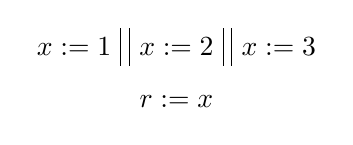
\begin{tikzpicture}
      \node (wxa) %[left of = mid, node distance = 1.1cm] 
        % at (0,1)
        {$x:=1$};

      \node (wxb) [right of = wxa, node distance = 1.3cm] 
        % at (1,1)
        {$x:=2$};

      \node (wxc) [right of = wxb, node distance = 1.3cm] 
        % at (2,1)
        {$x:=3$};

      \node (rx) [below of = wxb, node distance = 0.7cm] 
        % at (1,0)
        {$r:=x$};

      \draw ($(wxa.north east)$) -- ($(wxa.south east)$);
      \draw ($(wxb.north west)$) -- ($(wxb.south west)$);
      \draw ($(wxb.north east)$) -- ($(wxb.south east)$);
      \draw ($(wxc.north west)$) -- ($(wxc.south west)$);
\end{tikzpicture}
\end{center}


Under the interleaving semantics 
it has $3! = 6$ traces with each trace consisting of $4$ events,
as depicted on \cref{fig:intro-traces}.
Event themselves represent atomic side-effects 
of instructions' execution. In our case 
it is either a write of a value to a shared variable $\wlab{x}{a}$,
or a read of a particular value from a shared variable $\rlab{x}{a}$.  

\begin{figure}[h]
\footnotesize
\begin{center}
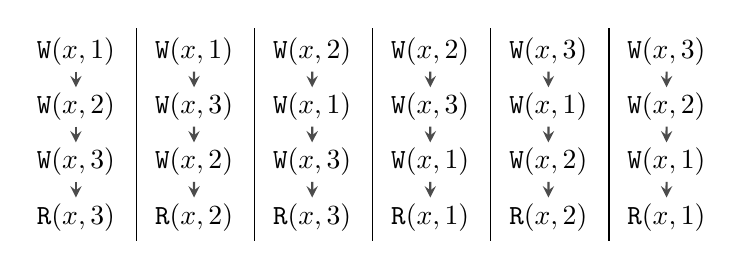
\begin{tikzpicture}[xscale=1.5, yscale=0.7]
    \node (wxaa) at (0,3) {$\wlab{x}{1}$};
    \node (wxab) at (0,2) {$\wlab{x}{2}$};
    \node (wxac) at (0,1) {$\wlab{x}{3}$};
    \node (rxa)  at (0,0) {$\rlab{x}{3}$};

    \draw[ca] (wxaa) -- (wxab);
    \draw[ca] (wxab) -- (wxac);
    \draw[ca] (wxac) -- (rxa);

    \draw ($(wxaa.north east) + (0.1,0)$) -- ($(rxa.south east) + (0.1,0)$);


    \node (wxba) at (1,3) {$\wlab{x}{1}$};
    \node (wxbb) at (1,2) {$\wlab{x}{3}$};
    \node (wxbc) at (1,1) {$\wlab{x}{2}$};
    \node (rxb)  at (1,0) {$\rlab{x}{2}$};

    \draw[ca] (wxba) -- (wxbb);
    \draw[ca] (wxbb) -- (wxbc);
    \draw[ca] (wxbc) -- (rxb);

    \draw ($(wxba.north east) + (0.1,0)$) -- ($(rxb.south east) + (0.1,0)$);

    \node (wxca) at (2,3) {$\wlab{x}{2}$};
    \node (wxcb) at (2,2) {$\wlab{x}{1}$};
    \node (wxcc) at (2,1) {$\wlab{x}{3}$};
    \node (rxc)  at (2,0) {$\rlab{x}{3}$};

    \draw[ca] (wxca) -- (wxcb);
    \draw[ca] (wxcb) -- (wxcc);
    \draw[ca] (wxcc) -- (rxc);

    \draw ($(wxca.north east) + (0.1,0)$) -- ($(rxc.south east) + (0.1,0)$);

    \node (wxda) at (3,3) {$\wlab{x}{2}$};
    \node (wxdb) at (3,2) {$\wlab{x}{3}$};
    \node (wxdc) at (3,1) {$\wlab{x}{1}$};
    \node (rxd)  at (3,0) {$\rlab{x}{1}$};

    \draw[ca] (wxda) -- (wxdb);
    \draw[ca] (wxdb) -- (wxdc);
    \draw[ca] (wxdc) -- (rxd);

    \draw ($(wxda.north east) + (0.1,0)$) -- ($(rxd.south east) + (0.1,0)$);

    \node (wxea) at (4,3) {$\wlab{x}{3}$};
    \node (wxeb) at (4,2) {$\wlab{x}{1}$};
    \node (wxec) at (4,1) {$\wlab{x}{2}$};
    \node (rxe)  at (4,0) {$\rlab{x}{2}$};

    \draw[ca] (wxea) -- (wxeb);
    \draw[ca] (wxeb) -- (wxec);
    \draw[ca] (wxec) -- (rxe);

    \draw ($(wxea.north east) + (0.1,0)$) -- ($(rxe.south east) + (0.1,0)$);

    \node (wxfa) at (5,3) {$\wlab{x}{3}$};
    \node (wxfb) at (5,2) {$\wlab{x}{2}$};
    \node (wxfc) at (5,1) {$\wlab{x}{1}$};
    \node (rxf)  at (5,0) {$\rlab{x}{1}$};

    \draw[ca] (wxfa) -- (wxfb);
    \draw[ca] (wxfb) -- (wxfc);
    \draw[ca] (wxfc) -- (rxf);

    % \draw ($(wxfa.north east) + (0.1,0)$) -- ($(rxf.south east) + (0.1,0)$);

\end{tikzpicture}
\caption{}
\label{fig:intro-traces}
\end{center}
\end{figure}

The same information can be encoded in a single 
event structure containing $6$ events in total
(see \cref{fig:intro-es}). 
In the event structure there are two types of edges 
between the events. The gray arrows $e_1 \arrowCA e_2$ 
represent the \emph{causality relation}, a 
partial order reflecting the causal relationship
between the atomic events of computation.
The red edges $e_1 \arrowCF e_2$ represent 
the \emph{conflict relation} which is 
a symmetric and irreflexive relation 
encoding mutually exclusive events.
Each particular trace can be extracted from the event structure
as a linearisation of some \emph{configuration}, 
that is a causally-closed and conflict-free 
subset of events. 

\begin{figure}[h]
    \begin{center}
    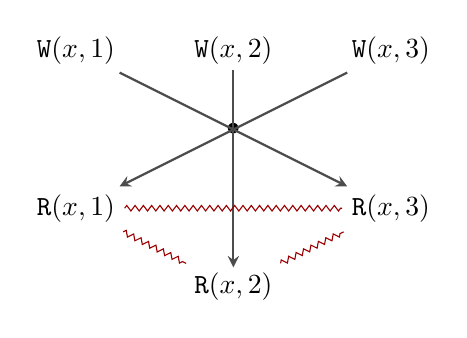
\begin{tikzpicture}[xscale=2]
        \node (wxa) at (0,1) {$\wlab{x}{1}$};
        \node (wxb) at (1,1) {$\wlab{x}{2}$};
        \node (wxc) at (2,1) {$\wlab{x}{3}$};
        \node (c)   at (1,0) {$\bullet$};
    
        \node (rxa) at (0,-1) {$\rlab{x}{1}$};
        \node (rxb) at (1, -2) {$\rlab{x}{2}$};
        \node (rxc) at (2,-1) {$\rlab{x}{3}$};
    
        \draw[ca] (wxa) -- (rxc);
        \draw[ca] (wxb) -- (rxb);
        \draw[ca] (wxc) -- (rxa);
    
        \draw[cf] (rxa) -- (rxb) -- (rxc);
        \draw[cf] (rxa) -- (rxc);
    \end{tikzpicture}
    %\caption{Event Structure}
    \label{fig:intro-es}
    \end{center}
    \end{figure}
    

In the programming language and formal semantics research community 
it becomes the de-facto standard to complement the theoretical 
studies with their mechanization in the \emph{proof assistants}
like Coq, Agda, Isabelle, Arend, and others,
as this process increases the reliability and reproducibility 
of the scientific results.
Yet, as far as we know, there is a little work on 
mechanization of event structures theory. 

Our work is aimed to close this gap. 
Our goal is to develop a Coq library containing 
a comprehensive set of common definitions, lemmas, 
and tactics that would allow the researchers 
to utilize the theory of event structures 
for the needs of their domain. 

In this work in progress report we sketch 
the common design princples behind our library
and give a concrete example of its usage  
by developing a formal mechanized semantics of simple 
register machine with shared memory. 
\section{Related Work}

Event structures were introduced by Winskel to study the semantics of 
the calculus of communicating systems~\cite{Winskel:86, Winskel:82}. 
Several modifications of event structures~\cite{Langerak:91, Boudol-Castellani:1991}
were later proposed to tackle similar problems.  
 
More recently, event structures were applied 
in the context of relaxed memory models~%
\cite{Jeffrey-Riely:LICS16, PichonPharabod-Sewell:POPL16, Chakraborty-Vafeiadis:POPL19, Moiseenko-al:ECOOP20}.
Among this line of work, we are aware of only one paper~\cite{Moiseenko-al:ECOOP20}
that was accompanied by a mechanisation in a proof assistant. 
The authors formalised \weakestmo~\cite{Chakraborty-Vafeiadis:POPL19} 
memory model in \coq. However, this memory model uses 
a custom variant of event structures, that does not 
obey axioms of any conventional class of 
event structures~\cite{Winskel:82, Langerak:91, Boudol-Castellani:1991}. 
This fact makes it harder to reuse and adapt it 
to other applications of the theory. 


\section{Background}

% In this section we give some background on event structures. 
There exist several modifications of events structures.
Currently we have implemented only 
the \emph{prime event structures}~\cite{Winskel:86} in our library. 
Below we give some background on this class of event structures. 

\begin{definition} 
\label{es_def}
A prime event structure (PES) is a triple $(\eventSet, \caOrd, \cfRel)$, where
\begin{itemize}
  \item E is a set of events
  \item $\caOrd$ is a causality relation on E such that 
  \begin{itemize}
    \item $ (\eventSet, \caOrd) $ is a partial order;
    \item for every $e \in \eventSet$ its causality prefix ${\prefix{e} := \{ e' : e' \caOrd e \}}$ 
      is finite, \ie every event is caused by a finite set of events.
  \end{itemize}
  \item $\#$ is a conflict relation on $E$ such that:
  \begin{itemize}
    \item $\#$ is irreflexive and symmetric;
    \item it satisfies the \emph{hereditary} condition:
    $$ \forall e_1, e_2, e_3 \in E \ldotp \ e_1 \cfRel e_2 \land e_2 \caOrd e_3 \Rightarrow e_1 \cfRel e_3 $$
      That is, if two events are in conflict, then all their causal successors 
      are necessarily in conflict.
  \end{itemize}
\end{itemize}
\end{definition}

A single prime event structures can encode multiple runs of a program.
Each individual run can be extracted as a \emph{configuration}. 
In other words, configurations are used to model 
a history of computation up to a certain point.

\begin{definition}
A configuration of PES $(E, \caOrd, \cfRel)$ is a set of events $X \subseteq E$ such that
\begin{itemize}
  \item it is causally closed 
    $$ \forall e_1, e_2 \in E \ldotp e_2 \in X \land e_1 \caOrd e_2 \Rightarrow e_1 \in X $$
  \item and conflict-free 
    $$ \forall e_1, e_2 \in X \ldotp \neg (e_1 \cfRel e_2) $$
\end{itemize}
\end{definition}

% We will also need a subclass of prime event structures --- 
% \emph{confusion-free} event structures~\cite{Nielsen-al:1981}. 
% In a confusion-free structure the conflict relation is generated from 
% a simpler \emph{primitive conflict} relation $\primcfRel$,
% which denotes pairs of events at which the computation
% diverges into two conflicting branches. 

% \begin{definition}
% Confusion-free event structures (CES) is a triple $(E, \caOrd, \primcfRel)$, where
% \begin{itemize}
%   \item $\caOrd$ obeys the same laws as for prime event structures;
%   \item $\primcfRel$ is a primitive conflict relation, such that
%   \begin{itemize}
%     \item it is irreflexive, symmetric and transitive;
%     \item it does not violate the hereditary condition:
%     $$ \forall e_1, e_2, e_3 \in E \ldotp 
%        e_1 \primcfRel e_2 \land e_2 \caOrd e_3 \Rightarrow \neg (e_1 \caOrd e_3) $$
%     \item it satisfies the axiom of \emph{choice locality}
%   \end{itemize}
%     $$ \forall e_1, e_2, e_3 \in E \ldotp e_1 \caOrd e_2 \land e_2 \primcfRel e_3 \Rightarrow e_1 \caOrd e_3 $$
% \end{itemize}
% \end{definition}

% From a confusion-free event structure one can construct a prime event structure
% by defining $\cfRel$ as follows:
% $$ e_1 \cfRel e_2 \iff 
%    \exists e'_1, e'_2 \in \eventSet \ldotp e'_1 \primcfRel e'_2 \land
%    e'_1 \caOrd e_1 \land e'_2 \caOrd e_2 $$

% It can be shown that the conflict relation defined in this way 
% satisfies the axioms of prime event structure.

% The following simple facts about prime event structures:

% \begin{lemma}
%   A set $\lceil e \rceil$ is conflict-free for any $e \in E$.
% \end{lemma}

% And a more general one:

% \begin{lemma}
%   A set $\lceil e \rceil$ is a configuration for any $e \in E$.
% \end{lemma}


\section{Overview}

In this section we sketch the design principles of our library. 

We build our mechanization on top of \mathcomp~\cite{Mahboubi-Tassi:MATHCOMP17} library 
using the \ssreflect~\cite{Gonthier-al:SSR2016} extension of the \coq system.
We also use the \emph{small-scale reflection} 
methodology~\cite{Gonthier-Assia:SSR2010, Gonthier-al:SSR2016}, 
a key ingredient of the \ssreflect. 

The small-scale reflection approach is based on 
pervasive use of symbolic representation of the proof goal, 
which \emph{relfects} the logical representation. 
The symbolic representation can be manipulated 
by the computational engine of the language, 
allowing the user to automate low-level routine 
proof management by using various decision 
and simplification procedures. 
Whenever the user needs to guide the proof 
it can switch to logical representation
and perform some proof steps manually. 

To achieve better automation one is recommended 
to use \emph{decidable} and \emph{computable} procedures
whenever possible.
For example, in the context of our library, 
we encode the binary relations of the event structures
as decidable \texttt{bool}-valued relations, 
\ie $\caOrd, \cfRel : E \fun E \fun \texttt{bool}$,
as opposed to \emph{propositional} 
relations of type $E \fun E \fun \texttt{Prop}$. 

We also favor the computational encoding of semantics. 
In the line of the recent related works on mechanization 
of operational semantics~\cite{Xia-al:POPL2019, Letan-al:CPP2020, Affeldt-al:ICMPC2019}, 
we encode the semantics as monadic interpreters.  
This allows us to extract~\cite{Letouzey:CCE2008} 
the semantics as a functional program and run it. 
We believe that the possibility to run the semantics 
is a very useful feature, as it allows 
to debug the formal semantics
and helps to develop better intuition about it.

Finally, we use yet another feature of \mathcomp --- 
\emph{packed classes}~\cite{Garillot-al:ICTPHOL2009}, 
in order to encode the algebraic hierarchy
of various classes of event structures. 
\section{Case Study}

In this section we provide a case study demonstrating 
an application of our mechanazied theory of event structures.
We show how it can be used to encode semantics of 
a parallel register machine equipped with a shared memory.

\subsection{Register Machine}

For our case study, we use a simple idealised model 
of a register machine, which consists of a finite 
sequence of instructions, an instruction pointer,
and an infinite set of registers. 
The syntax of the machine's language is 
shown in~\cref{fig:regmachine-syntax}.

\begin{figure}[h!]
\[
\begin{array}{rclclll}
  P &\in& \Prog   &::=& i_1 \seq \dots \seq i_n           & \text{program}                 \\

  I &\in& \Inst     &::=&                                 & \text{instruction}             \\
              & &   & | & \assignInst{r}{v}               & \text{assign to register}      \\
              & &   & | & \opInst{\otimes}{r_1}{r_2}{r_3}  & \text{apply binary operation}  \\
              & &   & | & \jumpInst{r}{\ip{i}}            & \text{conditional jump}        \\
              & &   & | & \exitInst                       & \text{exit}                    \\
              & &   & | & \readInst{r}{x}                 & \text{read from memory}        \\
              & &   & | & \writeInst{x}{v}                & \text{write to memory}         \\

  r      &\in& \Reg     &   &                    & \text{thread-local register}   \\ 
  x      &\in& \Loc     &   &                    & \text{shared memory location}  \\ 
  v      &\in& \Z       &   &                    & \text{value}                   \\
  \otimes&\in& \BinOp   &   &                    & \text{binary operation}        \\
  \ip{i} &\in& \N       &   &                    & \text{instruction label}       \\ 

\end{array}
\] 
\caption{Syntax of the register machine}
\label{fig:regmachine-syntax}
\end{figure}

We first present the semantics of a single-threaded program.
Under this semantics, memory access instructions 
do not operate on shared memory
but rather produce a \emph{label}
denoting the side-effect of the operation 
(see \cref{fig:label-syntax}).
This encoding allows us to decouple 
the semantics of the register machine 
from a \emph{memory model}.

\begin{figure}[h!]
\[
\begin{array}{rclclll}

  \ell &\in& \Lab  &::=&                                & \text{}             \\
              & &  & | & \rlab{x}{v}                    & \text{read of value $v$ from location $x$}   \\
              & &  & | & \wlab{x}{v}                    & \text{write of value $v$ to location $x$}    \\

\end{array}
\] 
\caption{Syntax of Labels}
\label{fig:label-syntax}
\end{figure}

The semantics is given in the form of a
\emph{labelled transition system}:~%
\footnote{As we have mentioned, in our \coq development we actually use 
the monadic encoding of the operational semantics. 
The labelled transition system can be derived from this encoding.}
$P \vdash s \thrdstep{l} s'$,
where $P$ is a program, $l$ is a label, $s$ and $s'$ are states of the machine. 
The state of the machine itself consists of an instruction pointer $\ip{i}$
and a map from registers to their values $\regmap$, 
as shown in \cref{fig:regmachine-thrdstate}. 
The rules of the semantics are standard 
(see \cref{fig:regmachine-thrdsem}).

\begin{figure}[h!]
\[
\begin{array}{rclclll}

  s          &\in& \ThrdState    &::=& \tup{\ip{i}, \regmap} &                         \\
  \ip{i}     &\in& \N            &   &                    & \text{instruction pointer} \\
  \regmap    &\in& \Reg \fun \Z  &   &                    & \text{register mapping}   \\

\end{array}
\] 
\caption{Thread state of register machine}
\label{fig:regmachine-thrdstate}
\end{figure}

\begin{figure*}[t]

  \begin{subfigure}{0.5\linewidth}
  \begin{center}

  \AXC{$P[\ip{i}] =\ \assignInst{r}{v}$}
  \RightLabel{\texttt{Assign}}
  \UIC{$P \vdash \tup{\ip{i}, \regmap} \thrdstep{\eps} \tup{\ip{i+1}, \updmap{\regmap}{r}{v}}$}
  \DisplayProof
  
  \rulevspace
  
  \AXC{$P[\ip{i}] =\ \writeInst{x}{v}$}
  \RightLabel{\texttt{Store}}
  \UIC{$P \vdash \tup{\ip{i}, \regmap} \thrdstep{\wlab{x}{v}} \tup{\ip{i}+1, \regmap}$}
  \DisplayProof
   
  \rulevspace
  
  \AXC{$P[\ip{i}] =\ \readInst{r}{x}$}
  \RightLabel{\texttt{Load}}
  \UIC{$P \vdash \tup{\ip{i}, \regmap} \thrdstep{\rlab{x}{v}} \tup{\ip{i+1}, \updmap{\regmap}{r}{v}}$}
  \DisplayProof

  \end{center}
  \end{subfigure}
  %
  \begin{subfigure}{0.5\linewidth}
  \begin{center}
    
  \AXC{$P[\ip{i}] =\ \opInst{\otimes}{r_1}{r_2}{r_3}$}
  \AXC{$v = \appmap{\regmap}{r_2} \otimes \appmap{\regmap}{r_3}$}
  \RightLabel{\texttt{Binop}}
  \BIC{$P \vdash \tup{\ip{i}, \regmap} \thrdstep{\eps} \tup{\ip{i+1}, \updmap{\regmap}{r_1}{v}}$}
  \DisplayProof

  \rulevspace

  \AXC{$P[\ip{i}] =\ \exitInst$}
  \AXC{$\len(P) = n$}
  \RightLabel{\texttt{Exit}}
  \BIC{$P \vdash \tup{\ip{i}, \regmap} \thrdstep{\eps} \tup{\ip{n}, \regmap}$}
  \DisplayProof

  \rulevspace

  \AXC{$P[\ip{i}] =\ \jumpInst{r}{\ip{j}}$}
  \AXC{$\appmap{\regmap}{r} = 0$}
  \RightLabel{\texttt{CJump}$_z$}
  \BIC{$P \vdash \tup{\ip{i}, \regmap} \thrdstep{\eps} \tup{\ip{i+1}, \regmap}$}
  \DisplayProof
  
  \rulevspace
  
  \AXC{$P[\ip{i}] =\ \jumpInst{r}{\ip{j}}$}
  \AXC{$\appmap{\regmap}{r} \neq 0$}
  \RightLabel{\texttt{CJump}$_{nz}$}
  \BIC{$P \vdash \tup{\ip{i}, \regmap} \thrdstep{\eps} \tup{\ip{j}, \regmap}$}
  \DisplayProof

  \end{center}
  \end{subfigure}

  \caption{Semantics of register machine}
  \label{fig:regmachine-thrdsem}
\end{figure*}



% \subsection{Shared Memory}
% \input{sharedmem-eventstruct.tex}

\section{Implementation}

\subsection{How we encode Event Structures}
% Как мы видели ранее в Step-by-step example наша стуркура событий содержит такие функции как frf fpred. Сами события это элементы некоторого множества E (множества итендификаторов), которое должно удволетворять следущим свойствам:
\begin{definition}[identifier set]
  $\mathcal{E}$ is an identifier set if:
  \begin{itemize}
    \item There is some $ident_0 \in \mathcal{E}$ ~--- first identifier
    \item $\mathcal{E}$ has well-founded partitial order $\leqslant_\mathcal{E}$
    \item There is some function, that takes some finite identifies set $E \subset \mathcal{E}$ and returns a fresh identifier. Formally: $fresh : \mathcal{P}_{fin}(\mathcal{E}) \to \mathcal{E}$, satisfies $$\forall e \in E, \ e <_\mathcal{E} fresh(E)$$
  \end{itemize}
\end{definition}
% Пусть E это множества всех событий программы тогда у нас есть
  $$\ffun{lab} : E \rightharpoonup \lb $$
% где label -- множество всех меток (таких как W(x, 5), R(y, 6), ThreadStart, ThreadEnd etc)
% Мы будем говорить что е это "read"-event c локацией х и значением i если lab(e) = R(x,i), аналогично "write"-event
% В итоге формально мы строим четверку
\begin{definition}[Execution Event Structure]
  $$exec\_event\_structure \ \triangleq \ \langle E, \ \ffun{lab}, \ \fpred, \ \frf \rangle$$
  where
  \begin{itemize}
    \item $E$ ~--- finite subset of some identifiers set $\mathcal{E}$
    \item $\fpred$ ~--- function that returns a predsessor (w.r.t. the program order) of event
    \item $\frf$ ~--- function that takes "read"-event $e$ and returns a "write"-event from witch $e$ reads
    \item $\ffun{lab} : E \to \lb$ ~--- function that returns event's label
  \end{itemize}
  Also we require
  \begin{itemize}
    \item $\forall e \in E, \ \fpred(e) \leqslant_E e$ and $\frf(e) \leqslant_E e$
    \item $\forall e_1 \ e_2 \in E, \ e_2 = \frf(e_1) \ \Leftrightarrow \ e_1$ is a "read"-event and $e_2$ is a "write"-event with the same location and value
  \end{itemize}
\end{definition}
  
% Далее для простоты будем отождествлять иденфикаторы с их метками, а Execution Event Structure с их множеством итендификаторов

% Теперь наша задача: определить в этих терминах простые структуры событий. Для этого надо определить частичный порядок <= и отношение конфликта #
% Начнем с отношения causality. В нашей статье мы будем считать, что событие e1 влечет событие e2 если 
\begin{itemize}
  \item Programm instruction, that corresponds to event $e_1$ states before the programm instruction, that corresponds to $e_2$
  \item Or $\ e_2$ is the "read"-event and it reads from "write"-event $e_1$
\end{itemize}
% Или формально:
\begin{itemize}
  \item $\fpred(e_1) \ =\ e_2$
  \item Or $\ \frf(e_1) \ =\ e_2$
\end{itemize}
% Любую функцию f можно считать отношением
  $$ a \ f \ b \ \triangleq\ f(a) \ = \ b$$
% Имея ввиду обозначение выше определим
\begin{definition}[causality relation]
  $$\leqslant \ \triangleq \ (\fpred \cup \frf)^* $$
\end{definition}
% Заметим, что в множестве E уже есть тотальный порядок $\leqslant_E$. Нетрудно видеть что полученнле отношение casuality является его предпорядком [смотри Well-foundedness and monads]
\begin{lemma}
  If $\leqslant$ is a casuality order of $E$ then $\leqslant \ \subset \ \leqslant_E$
\end{lemma}
% Теперь давайте определим отношение конфликта. Посмотрев на отношение конфликта в определении СС [ссылка], мы можем установить следущий факт
\begin{lemma}\label{lma_confl}
  If $\ e_1 \leqslant e_2, \ e_3 \leqslant e_4$ and $e_1 \# e_3$ holds then $e_2 \# e_4$
\end{lemma} 
% То есть отношение конфликта должно "протаскиваться" через отношение <=. Наша интуиция будет заключаться в том, что мы определим "минимальное" отношение конфликта, замкнув, котрое по свойству консистентности [ссылка] мы получим полное отношение #. 
% И так откуда берутся конфликты? [тут должен был заход через Step-by-step example]. 
% И так мы видим, что если у событий есть общий предок (относительно отношения fpred) то эти события происходят в двух разных выполнениях программы и, соответвенно находятся в отношении конфликта
\begin{definition}[immediate conflict relation]
  $$ e_1 \, \ffun{icf} \, e_2 \ \triangleq\ \exists e, \, e = \fpred(e_1) = \fpred(e_2)  $$
\end{definition}
% Далее можно определить отношение конфликта как консистентное замыкание icf
\begin{definition}[conflict relation]
  $$ e_1 \, \# \, e_2 \ \triangleq\ \exists e_3\, e_4, e_3 \, \ffun{icf} \, e_4 \ and \ e_3 \leqslant e_1, \, e_4 \leqslant e_2 $$
\end{definition}
% Однако с этим определением возникает одна проблема. Понятно что отношение определенное таким образом получается симметричным и консистентным. Будет ли оно иррефлексивность? Оказывается, что в общем случае нет. Рассмотрим следущую программу:
\begin{figure}[h]
  \begin{center}
    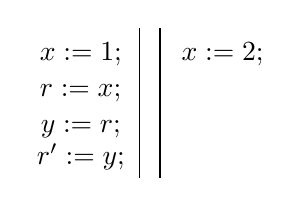
\begin{tikzpicture}

      \node (iwy) %[left of = mid, node distance = 1.1cm] 
      at (-1.3, 2.5)
      {$x:=1;$};
    
      \node (irx) [above = -0.5cm of iwy.west, anchor = west] 
      {$r:=x;$};
    
      \node (iwx) %[right of = mid, node distance = 0.8cm] 
       at (0.5, 2.5)
      {$x:=2;$};
    
      \node (iwz) %[right of = mid, node distance = 0.8cm] 
      at (-1.3, 1.55)
     {$y:=r;$};
    
     \node (iww) %[right of = mid, node distance = 0.8cm] 
      at (-1.3, 1.2)
     {$r':=y;$};
    
      \draw ($ (iwy.south east) + (0.1,-1.3) $) -- ($ (iwy.south east) + (0.1,0.6) $);
      \draw ($ (iwx.south west) + (-0.15,-1.3) $) -- ($ (iwx.south west) - (0.15,-0.6) $);
    \end{tikzpicture}
  \end{center}
\end{figure}
% Давайте как в Step-by-step example построим по шагам фрагмент соответвующей этой программе exec_event_structure до чтения из y
\begin{figure}[h]
  \begin{center}
    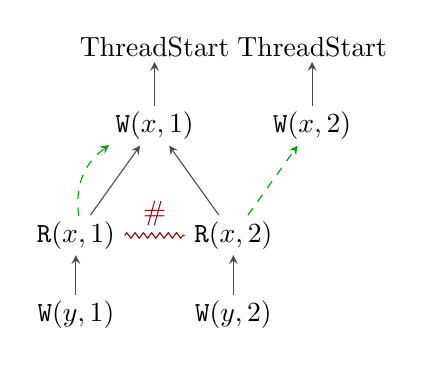
\begin{tikzpicture}
      \node (ts1) at (-3,1.2) {ThreadStart};
      \node (ts2) at (-1, 1.2) {ThreadStart};
      \node (wxo) at (-3,0.2) {$\wlab{x}{1}$};
      \node (wxt) at (-1,0.2) {$\wlab{x}{2}$};
      \node (rxt) at (-2, -1.2) {$\rlab{x}{2}$};
      \node (rxo) at (-4, -1.2) {$\rlab{x}{1}$};
      \node (wyo) at (-4, -2.2) {$\wlab{y}{1}$};
      \node (wyt) at (-2, -2.2) {$\wlab{y}{2}$};
      \draw[po] (wxo)  --  (ts1);
      \draw[po] (wxt)  --  (ts2);
      \draw[po] (rxt)  --  (wxo);
      \draw[rf] (rxt)  --  (wxt);
      \draw[po] (rxo)  --  (wxo);
      \draw[rf] (rxo)  edge[bend left] (wxo);
      \draw[cf] (rxo)  -- node[above]{$\#$}  (rxt);
      \draw[po] (wyo) -- (rxo);
      \draw[po] (wyt) -- (rxt);
    \end{tikzpicture}
  \end{center}
\end{figure}
% Видно что наша программа в первом потоку разделилась на два независимых выполнения: выполнение в котором мы прочитали из x 1 (обозначим за выболнение (а)) и выполненние в котором прочитали из х 2 (выполнение (b))
%Теперь мы хотим добавить в нашу структуру событий чтение в y. посмотрим что будет если прочитать при выполнении (а) в у 2 (то есть запись из (b))
\begin{figure}[h]
  \begin{center}
    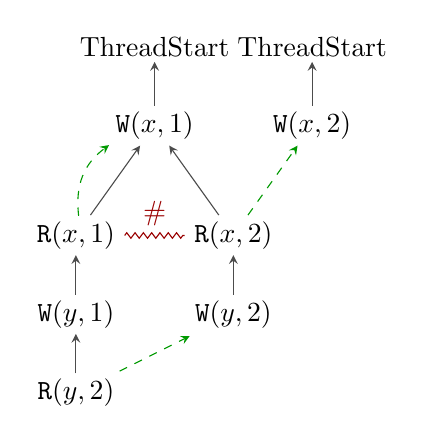
\begin{tikzpicture}
      \node (ts1) at (-3,1.2) {ThreadStart};
      \node (ts2) at (-1, 1.2) {ThreadStart};
      \node (wxo) at (-3,0.2) {$\wlab{x}{1}$};
      \node (wxt) at (-1,0.2) {$\wlab{x}{2}$};
      \node (rxt) at (-2, -1.2) {$\rlab{x}{2}$};
      \node (rxo) at (-4, -1.2) {$\rlab{x}{1}$};
      \node (wyo) at (-4, -2.2) {$\wlab{y}{1}$};
      \node (wyt) at (-2, -2.2) {$\wlab{y}{2}$};
      \node (ryt) at (-4, -3.2) {$\rlab{y}{2}$};
      \draw[po] (wxo)  --  (ts1);
      \draw[po] (wxt)  --  (ts2);
      \draw[po] (rxt)  --  (wxo);
      \draw[rf] (rxt)  --  (wxt);
      \draw[po] (rxo)  --  (wxo);
      \draw[rf] (rxo)  edge[bend left] (wxo);
      \draw[cf] (rxo)  -- node[above]{$\#$}  (rxt);
      \draw[po] (wyo) -- (rxo);
      \draw[po] (wyt) -- (rxt);
      \draw[po] (ryt) -- (wyo);
      \draw[rf] (ryt) -- (wyt);
    \end{tikzpicture}
  \end{center}
  \caption{}
  \label{fig:cf}
\end{figure}
We have $\rlab{x}{1} \leqslant \rlab{y}{2}$, $ \rlab{x}{2} \leqslant \rlab{y}{2}$ and $\rlab{x}{1} \ \# \ \rlab{x}{2}$. Thus $\rlab{y}{2} \ \# \ \rlab{y}{2}$ holds (see~\cref{lma_confl})
% Но отношение конфликта должно быть иррефлексивным. Заметим, однако, что (a) и (b) не могут произойти при одном исполнении программы, а значит и чтения R(y,2) из W(y,2) тут быть не должно, полная структура событий тут должна выглядеть так:
\begin{figure}
  \begin{center}
    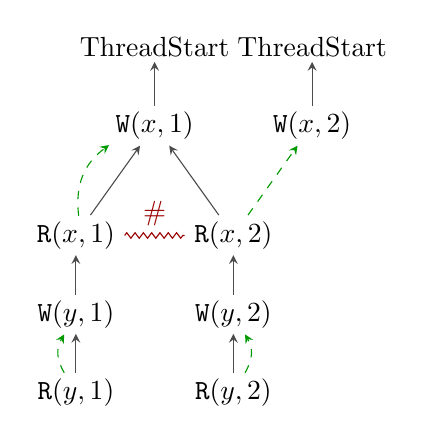
\begin{tikzpicture}
      \node (ts1) at (-3,1.2) {ThreadStart};
      \node (ts2) at (-1, 1.2) {ThreadStart};
      \node (wxo) at (-3,0.2) {$\wlab{x}{1}$};
      \node (wxt) at (-1,0.2) {$\wlab{x}{2}$};
      \node (rxt) at (-2, -1.2) {$\rlab{x}{2}$};
      \node (rxo) at (-4, -1.2) {$\rlab{x}{1}$};
      \node (wyo) at (-4, -2.2) {$\wlab{y}{1}$};
      \node (wyt) at (-2, -2.2) {$\wlab{y}{2}$};
      \node (ryo) at (-4, -3.2) {$\rlab{y}{1}$};
      \node (ryt) at (-2, -3.2) {$\rlab{y}{2}$};
      \draw[po] (wxo)  --  (ts1);
      \draw[po] (wxt)  --  (ts2);
      \draw[po] (rxt)  --  (wxo);
      \draw[rf] (rxt)  --  (wxt);
      \draw[po] (rxo)  --  (wxo);
      \draw[rf] (rxo)  edge[bend left] (wxo);
      \draw[cf] (rxo)  -- node[above]{$\#$}  (rxt);
      \draw[po] (wyo) -- (rxo);
      \draw[po] (wyt) -- (rxt);
      \draw[po] (ryo) -- (wyo);
      \draw[rf] (ryo) edge[bend left] (wyo);
      \draw[po] (ryt) -- (wyt);
      \draw[rf] (ryt) edge[bend right] (wyt);
    \end{tikzpicture}
  \end{center}
\end{figure} \\
% Будем говорить, что сткуктура собырий консистентна если там нет чтений из конфликтующийх с ними записей. Формально
\begin{definition}[consistent Execution Event Structure]
  $$consitent\langle E, \ffun{lab}, \fpred, \frf \rangle \ \triangleq \ \forall e \in E, \ \neg (e \ \# \ \frf e)$$
\end{definition}
% Оказывается этого достатчно чтоб отношение конфликта было иррефлексивным
\begin{lemma}
  Let $E$ be a consistent Execution Event Structure (denote as $cexec\_event\_structure$). Then it's conflict relation $\#$ is irreflexive
\end{lemma}
% Получается что из консистентной exevstr можно получить ПCC
\subsection{Transitive Closure of Covering Function}

\todo{Sketch the problem of transitve closure termination 
and our solution if we'll have space and time}

% Initially, we used $\mathtt{nat}$ type to model event structures,
% but later we realised that using an arbirary well-founded set as a 
% domain of our model is a good generalisation for our results. 

% However, here arises one problem: we need the operation of 
% reflexive-transitive closure on binary relations over 
% general well-founded type, but $\mathtt{mathcomp}$ doesn't
% have it for them.

% So, we introduce our definition of transitive closure for a 
% decreasing function:

% \begin{definition}
%   Let $f : T \to \mathtt{seq} \ T$ be a decreasing function from 
%   well-founded set $T$ to lists of elements of $T$. Then the 
%   transitive closure of this function is the function 
%   $(\mathtt{suffix} \ f)$ from $T$ to lists of elements 
%   of $T$ such that for any $x : T$ the list $\mathtt{suffix} \ f \ x$
%   contain $f \ x$ and all elements of closures of elements of $f \ x$.
% \end{definition}

% Here, well-foundedness of $T$ guarantees that the process of the 
% calculation of the closure is finite for every element.

% Also, from this definition it is easy to see, that we can easily 
% generate binary relation on $T$, that corresponds to the closure:
% $$x \leq y \Leftrightarrow x \in \mathtt{suffix} \ f \ y.$$

% We also introduce a reflexive-transitive closure definition by 
% addition of element itself to its $\mathtt{suffix}$ list.

% For these definition we proved their correctness, i.e. we proved
% that the relation generated from our definition can be reflected 
% to the traditional Coq's inductive definition of the closure.

% Currently, we are working on the generalisation of the initial 
% function for $\mathtt{seq}$ to an arbitrary function 
% $f : T \to M \ T$, where M is such a monad, that there is a monad 
% morphism from $M$ to the list monad.

% This monad morphism allows us to use $\texttt{in}$ notation for
% monads by passing values to lists.

% For this problem we use $\mathtt{monae}$ Coq library, that 
% contains a hierarchy of monads. Using this library we defined
% monad morphisms for arbitrary monads and its special case for 
% failure monads.

\subsection{Construction small-step semantics}
Consider we have some Execution Event Structure $es = \la E, \ffun{lab}, \fpred, \frf \ra$, $pr \in E$ ~--- the $es$'s event and some fresh identifier $e = fresh(E)$. Let's define expansion $es$ with the event $e$ depending on its label:
\begin{definition}[Add event]
  \begin{itemize}
    \item $es + \la \wlab{x}{i}, \ pr \ra \ \triangleq \vspace{1mm} \\ \ 
    \la E \cup \{e\}, \
        \ffun{lab}[e \leftarrow \wlab{x}{i}], \
        \fpred[e \leftarrow pr], \
        \frf \ra\ $
        \vspace{1mm}
    \item $es + \la \text{ThreadStart} \ra \ \triangleq \vspace{1mm} \\
    \la E \cup \{e\}, \
    \ffun{lab}[e \leftarrow \text{ThreadStart}], \
    \fpred, \
    \frf \ra\ $
    \vspace{1mm}
    \item $es + \la \rlab{x}{i}, \ pr, \ wr \ra \ \triangleq$
    $$\la E \cup \{e\}, \
    \ffun{lab}[e \leftarrow \rlab{x}{i}], \
    \fpred[e \leftarrow pr], \
    \frf[e \leftarrow wr] \ra\ $$
  \end{itemize}
\end{definition}
Then we define programm configuration:
\begin{definition}[configuration]
  $$config \ \triangleq \ \la \es, \tmap \ra$$
  where
  \begin{itemize}
    \item $\es$ ~--- our current consistent Execution Event Structure
    \item $\tmap$ ~--- mapping from events in $\es$ to the pair of corresponding [TODO]
  \end{itemize}
\end{definition}

By $\es.E$, $\es.\ffun{lab}$, $\es.fr$ we denote $E$, $\ffun{lab}$ and $fresh(E)$ respectively, where $\es = \la E, \ffun{lab}, \fpred, \frf \ra$. Also by $\es.tid$ we denote the smallest number of thread that wasn't started yet. \\
If we have some $p : \texttt{P}$, and $t \in \mathbb{N}$ ~--- thread number, $p[t] :=$ $t$'s thread of programm $p$. 

Also we will need 'can-read-from relation':
\begin{definition}[Can-read-from relation]
  If $l, l' \in \lb$ we can define
  $$ l \ll l' \ \triangleq \ l = \rlab{x}{i} \ \text{and} \ l' = \wlab{x}{i}$$
\end{definition}

\subsection{Construction small-step semantics}
Consider we have some Execution Event Structure $es = \la E, \ffun{lab}, \fpred, \frf \ra$, $pr \in E$ ~--- the $es$'s event and some fresh identifier $e = fresh(E)$. Let's define expansion $es$ with the event $e$ depending on its label:
\begin{definition}[Add event]
  \begin{itemize}
    \item $es + \la \wlab{x}{i}, \ pr \ra \ \triangleq \vspace{1mm} \\ \ 
    \la E \cup \{e\}, \
        \ffun{lab}[e \leftarrow \wlab{x}{i}], \
        \fpred[e \leftarrow pr], \
        \frf \ra\ $
        \vspace{1mm}
    \item $es + \la \text{ThreadStart} \ra \ \triangleq \vspace{1mm} \\
    \la E \cup \{e\}, \
    \ffun{lab}[e \leftarrow \text{ThreadStart}], \
    \fpred, \
    \frf \ra\ $
    \vspace{1mm}
    \item $es + \la \rlab{x}{i}, \ pr, \ wr \ra \ \triangleq$
    $$\la E \cup \{e\}, \
    \ffun{lab}[e \leftarrow \rlab{x}{i}], \
    \fpred[e \leftarrow pr], \
    \frf[e \leftarrow wr] \ra\ $$
  \end{itemize}
\end{definition}
Then we define programm configuration:
\begin{definition}[configuration]
  $$config \ \triangleq \ \la \es, \tmap \ra$$
  where
  \begin{itemize}
    \item $\es$ ~--- our current consistent Execution Event Structure
    \item $\tmap$ ~--- mapping from events in $\es$ to the pair of corresponding [TODO]
  \end{itemize}
\end{definition}

By $\es.E$, $\es.\ffun{lab}$, $\es.fr$ we denote $E$, $\ffun{lab}$ and $fresh(E)$ respectively, where $\es = \la E, \ffun{lab}, \fpred, \frf \ra$. Also by $\es.tid$ we denote the smallest number of thread that wasn't started yet. \\
If we have some $p : \texttt{P}$, and $t \in \mathbb{N}$ ~--- thread number, $p[t] :=$ $t$'s thread of programm $p$. 

Also we will need 'can-read-from relation':
\begin{definition}[Can-read-from relation]
  If $l, l' \in \lb$ we can define
  $$ l \ll l' \ \triangleq \ l = \rlab{x}{i} \ \text{and} \ l' = \wlab{x}{i}$$
\end{definition}

\input{fig/small_step.tex}
[TODO: small step rules explanation]

[TODO: small step rules explanation]


\section{Future Work}

There are several directions for future work. 

First, we plan to apply our library to a wider range of problems. 
We are going to develop a mechanized semantics of some classical 
languages used to model concurrency, in particular 
the calculus of communicating systems~(CCS)~\cite{Milner:80} and 
$\pi$-calculus~\cite{Milner:99}.      
We also plan to continue our work on 
expressing various relaxed models of shared memory 
in terms of event structures.  

Second, we want to cover other classes of event structures in our library, 
in particular bundle~\cite{Langerak:91}, flow~\cite{Boudol-Castellani:1991}
and stable~\cite{Winskel:82, Winskel:86} event structures.
We plan to use them to develop mechanized \emph{denotational} semantics 
of concurrent languages and relaxed shared memory models.  

Finally, we plan to mechanize in Coq classical results 
that connect various classes of event structures  
by isomorphishm of configurations~\cite{Nielsen-al:1981, Boudol-Castellani:1991}. 
It will allow to easily establish the connection between operational and denotational 
semantics of concurrent languages.


\bibliography{main} 
\bibliographystyle{ieeetr}


\end{document}
